\chapter{Data Analysis}
In the analysis of experimental data, the primary goals are to extract the $2n$ removal cross section in the ${}^{17}\text{B} \to {}^{15}\text{B} + 2n$ reaction and to obtain the Relative energy spectrum. To achieve this, I will describe the procedure of identifying the secondary beam of ${}^{17}$B, and \textcolor{black}{selecting events involving the fragment ${}^{15}$B and two neutrons. Particular emphasis is placed on the process of selecting two-neutron events and the rejection of cross-talk.} The flow of the Data Analysis is as follows.

\begin{center}
    \begin{enumerate}[noitemsep]
        \item Select the event containing ${}^{17}$B beam by beam PID
        \item Select the event containing ${}^{15}$B fragment by fragment PID
        \item Select the event containing two neutron by cross-talk analysis
        \item Extract the 2n removal cross section of the ${}^{17}\text{B} \to {}^{15}\text{B} + 2n$ reaction
        \item Reconstruct Invariant Mass at target and obtain the Relative energy spectrum 
    \end{enumerate}
\end{center}

\section{Secondary Beam Particle Identification}
The primary beam was generated by the SRC, RIBF. By accelerating ${}^{48}$Ca to 345 MeV/u and bombarding it on a thick Be target (30mm), a secondary beam was produced. The characteristics of the primary beam is in Table \ref{tab:Primary_Beam}.

    \begin{table}[h]
        \centering 
            \begin{tabular}[]{c|c|c|c}
                \hline
                Primary Beam & Beam Energy & Beam Intensity & Primary Target  \\
                \hline 
                ${}^{48}$Ca & 345 MeV/u & 210 pnA & Be (30mm)\\
                \hline    
            \end{tabular}
        \caption{Information of Primary Beam}
        \label{tab:Primary_Beam}
    \end{table}

    \indent The collision of the initial beam and the target created the secondary beam, including not only purpose isotope of this experiment, ${}^{19}$B, but also other neighboring isotopes. The main isotope used in this research is ${}^{17}$B, which needed to be separated and identified through the BigRIPS separator. The identification of the ${}^{17}$B secondary beam was performed using the TOF-B$\rho$-$\Delta$E method. The identified ${}^{17}$B was then transferred to SAMURAI, where it underwent Coulomb dissociation, the main objective of this research. Three different targets were used: C, Pb, and Empty. The details for ${}^{17}$B with each target were as follows.

    \begin{table}[ht]
        \centering
        \begin{tabular}[ht]{c|c|c}
            \hline
            isotope & Target & Average Energy at the middle of target \\
            \hline
            & C (1.789 g/cm2)  & 270 MeV/u\\
            ${}^{17}$B & Empty  & 275 MeV/u\\
            & Pb (3.255 g/cm2) & 270 MeV/u\\
            \hline    
        \end{tabular}
        \caption{Information of Secondary Beam}
    \end{table}


\subsection{Analysis of Time of Flight}
The Time-of-Flight (TOF) is calculated using the time difference between two plastic scintillators. Three plastic scintillators are used for this TOF calculation. One is located at F7 and the other two, called SBT1 and SBT2, are at F13. The TOF between F7 and F13 is defined as following.
    \begin{align}
        \text{TOF}_{\text{F7-F13}} = \frac{t_{\text{SBT1}} + t_{\text{SBT2}}}{2} - t_{\text{F7}} + \Delta t_{offset}
    \end{align}
$\Delta t_{offset}$ is the offset used to correct for the difference between the actual measured $\text{TOF}_{\text{F7-F13}}$ and the TOF value calculated by considering the material between F7 and F13. For the calculation, runs with the f5 slit narrowed to $\pm$ 1mm (run number 428,429,431) are used,for the mono-energetic isotopes. The calculated $\text{TOF}_{\text{F7-F13}}$ value is 192.333 ns, and the corresponding $\Delta t_{offset}$ value is 172.025 ns.

\subsection{Analysis of Magnetic Rigidity}
Magnetic Rigidity $B\rho$ is derived by Beam Projection Chamber (BPC) located at F5 dispersive focal plane. The x position of a beam passing through F5 is measured by BPC, and the $B\rho$ is calculated using the following equation.
    \begin{align}
        B\rho = (1+\frac{x}{D}) B\rho_{0} 
    \end{align}
with the rigidity of the central trajectory $B\rho_{0}$ is 8.78 Tm, and  momentum dispersion $D$ is 3300 cm/$\%$. 

\subsection{Analysis of Energy Loss}
The energy loss $\Delta$E is measured in the Ionize Chamber for Beam (ICB). The correlation between $\Delta$E and Z can be obtained according to the simplified Bethe-Bloch's Energy loss formula as follows. In this formula, the \textit{density effect} correction $\delta$ or \textit{shell} correction $C$ are skipped.
    \begin{align}
        \frac{dE}{dx} = 2\pi N_{a} r_{e}^{2} m_{e} c^{2} \rho_{\text{P10}} 
        \bigg( \frac{Z_{\text{P10}}}{A_{\text{P10}}} \bigg) \bigg( \frac{Z^{2}}{\beta^{2}} \bigg) 
        \left[ \ln \frac{2m_{e}c^{2}\beta^{2}\gamma^{2}}{I_{\text{P10}}} - \beta^{2}  \right]
    \end{align}
with
    \begin{align}
        2 \pi N_{a} r_{e}^{2} m_{e} c^{2} \rho_{\text{P10}} = 0.307075 \text{ MeV cm}^{2} \text{g}^{-1} 
    \end{align}
    \begin{adjustwidth}{1cm}{}
        $N_{a}$ : Avogadro's number = 6.022 $\times$ 10$^{23}$\\
        $r_{e}$ : classical electron radius = 2.817 $\times$ 10$^{-13}$ cm\\ 
        $m_{e}$ : electron mass = 0.511 MeV/c$^{2}$\\
        $\rho_{\text{P10}}$ : density of the P10 gas = 1.84 $\times$ 10$^{-3}$ g/cm$^{3}$\\
        $Z_{\text{P10}}$ : effective atomic number of the P10 gas\\
        $A_{\text{P10}}$ : effective mass number of the P10 gas\\
        $I_{\text{P10}}$ : mean excitation energy of the P10 gas\\ 
        $\beta$ = $v / c$ of the beam particle\\
        $\gamma$ = $1 / \sqrt{1-\beta^{2}}$
    \end{adjustwidth}
\vspace{3mm}
Since the P10 gas is compound of 90$\%$ Ar and 10$\%$ CH$_{4}$, the mean excitation energy $I_{\text{P10}}$ is calculated as follows. The detail of the calculation of I for compound material is described in the Appendix A.

\subsection{Beam Particle Identification}
Secondary beam particles are identified using the TOF-B$\rho$-$\Delta$E method. TOF is calculated from time difference between scintillator at F7 and F13, B$\rho$ is calculated from the beam passing x position at F5, and $\Delta$E is measured from ionization chamber ICB. A/Z and Z is driven by the following equation.
\begin{align}
    \beta_{\text{TOF}} &= L(\text{F7-F13}) / ( {\text{TOF}}_{\text{F7-F13}} \times c )\\
    \beta_{\text{F5}} &= f(\text{TOF}_{\text{F7-F13}})\\
    A/Z &= c B\rho_{\text{F5}} \gamma_{\text{F5}} / m_u \beta_{\text{F5}}
\end{align}
\begin{align}
    &\Delta x = (51-0.0262)*0.9*0.0016608 + (51-0.0262)*0.1*0.000667 \\
    &Z = \beta \sqrt{\Delta E_{\text{ICB}}/\{0.307075 \cdot \Delta x \cdot (Z_{\text{P10}}/A_{\text{P10}}) \cdot \ln( 2m_{e}c^{2}\beta^{2}\gamma^{2}/I_{\text{P10}} - \beta^{2})\}}
\end{align}
 $f(\text{TOF}_{\text{F7-F13}})$ is polynomial function of TOF for fitting $\beta$. $\Delta E_{\text{ICB}}$ is total energy loss at ICB and $\Delta x$ is the travel distance in ICB, which is calculated as (total length - wire length) * (probability of each gas in P10) * (volume density).
Figure \ref{fig:Beam_PID} shows the histogram of particle identification of the secondary beam with x-axis as A/Z and y-axis as Z. The statistic of secondary beam for each target is in Table \ref{tab:Beam_PID}.

\begin{figure}[h]
    \centering
    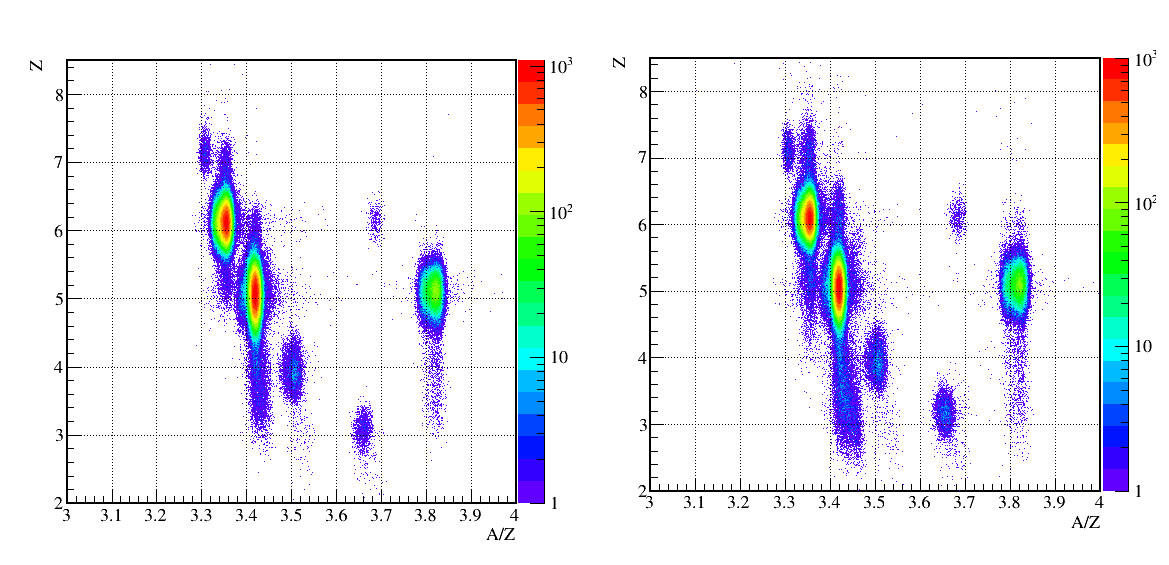
\includegraphics[width=\textwidth]{chapter4/beampid.png}
    \caption[Secondary Beam Particle Identification]{Beam Particle Identification for Pb target (left) and C target (right)}
    \label{fig:Beam_PID}
\end{figure}

\begin{table}[h]
    \centering
    \begin{tabular}{cccc}
        \hline
        Secondary Beam & Pb target & C target & Empty target\\             
        \hline \hline
        ${}^{17}$B & 829586 & 756021 & 331445 \\
        ${}^{19}$B &  160905&  144243&  63033\\
        ${}^{20}$C &  1675080 & 1483113 & 510410 \\
        \hline
    \end{tabular}
    \caption{Statistic of Secondary Beam}
    \label{tab:Beam_PID}
\end{table}

%----------------------------------------------------------------------------------------------------

\section{Beam Profile at Target}

The beam profile at the target can be determined using two drift chambers, BDC1 and BDC2, located upstream of the target. BDC1 and BDC2 are Ionized Drift Chambers that allow for the determination of a particle's trajectory through reconstruction of the hit positions on each layer. By using this feature, the incident position and angle at the each BDC can be determined, and these are then extrapolated to find the incident position and angle at the target.

\subsection{BDC Calibration}
The BDC drift chamber is designed for getting the trajectory information of incident particle. Beam particle trajectory is obtained by following procedure.

\begin{enumerate}
    \item Get a STC function by integrating of TDC distribution.
    \item Get a hit position of each layer from drift time by STC function.
    \item Fit the trajectory with the linear function by the least-square method.
    \item Evaluate the resolution by the tracking residue distribution.
\end{enumerate}

\subsubsection{TDC Distribution}
The timing information of the BDC is obtained by TDC (Time-to-digital Converter). In figure \ref{fig:TDC_BDCs}, the TDC distribution of BDC1 and BDC2 are shown. Since we used common stop mode to take a TDC data in this experiment, the drift time is,
\begin{align}
    t_{drift} = t_{max} - t_{TDC}
\end{align}

where $t_{max}$ is the maximum TDC value. This TDC distribution is obtained from run 431 which set f5 slit is $\pm$ 5mm. Table \ref{tab:TDC_BDCs} shows the TDC window (minimum and maximum channel) condition of BDCs.

\begin{figure}
    \centering
    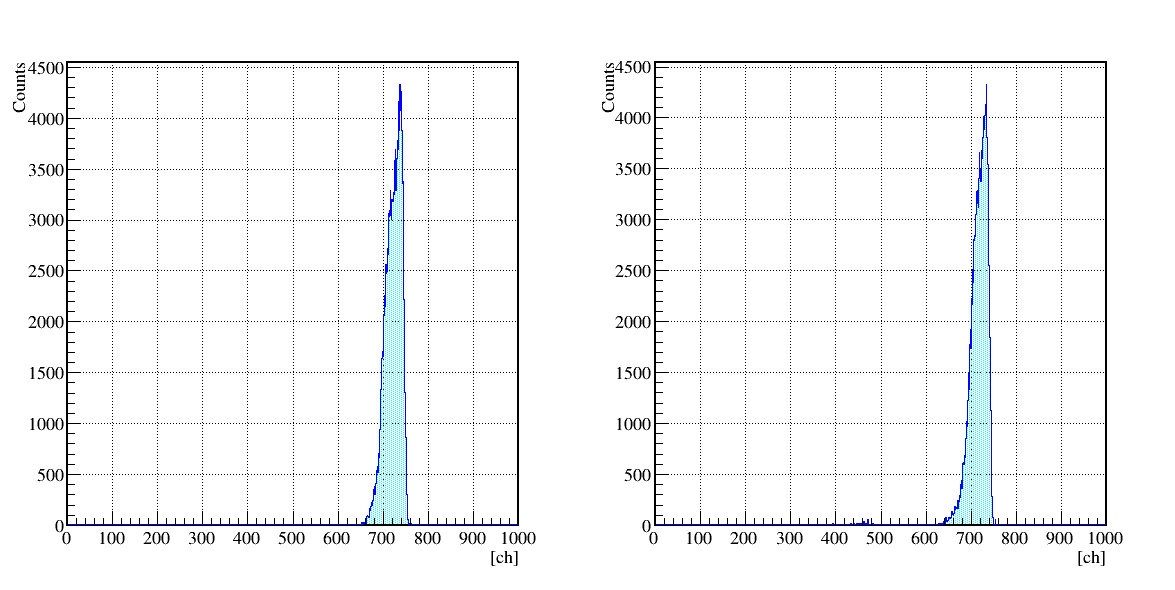
\includegraphics[width=14cm]{chapter4/tdc_bdcs.png}
    \caption[TDC Distribution of BDCs]{TDC Distribution of BDC1 (left) and BDC2 (right)}
    \label{fig:TDC_BDCs}
\end{figure}

\begin{table}[h]
    \centering
    \begin{tabular}{c|cc}
        \hline
        &$t_{min}$ [ch]&$t_{max}$ [ch]\\
        \hline
        BDC1&600&800\\
        BDC2&600&800\\        
        \hline
    \end{tabular}
    \caption[TDC Window Condition of BDCs]{TDC Window Condition of BDC1 and BDC2}
    \label{tab:TDC_BDCs}
\end{table}

\subsubsection{STC (Space to Time Conversion) Function}
By STD (Space to Time Conversion) function, the distance between hit position to anode wire can be calculated from drift time. STC (Space-Time Conversion) function assumed that the number of event is uniformly distributed in each drift length cell,  
\begin{align}
    \frac{dN}{dx} = const.  
\end{align}
Then STC function is derived by integrating the drift time distribution as,
\begin{align}
    &\frac{dN}{dt} \cdot \frac{dt}{dx} = const.\\
    &dx = C \cdot \frac{dN}{dt} \cdot dt,\\
    &x(t) = C \cdot \int_{t_{0}}^{t} \frac{dN}{dt} dt
\end{align}

where, C is normalization factor, $t_0$ is the minimum drift time and $t$ is the drift time from TDC distribution. 

\subsubsection{Linear fitting of trajectory}
After getting the STD function, the hit position of each layer is calculated from drift time as (4.14). Now we can get the trajectory of beam particle by fitting the hit position with linear function. When fitting the trajectory, the least-square method is used. The least-square method is the method of finding the best fit of a set of hit positions by minimizing the $\chi^2$ value. The $\chi^2$ value is defined as,
\begin{align}
    \chi^2 = \sum_{i=1}^{N} \frac{(x_{i} - f(x_{fit}))^2}{\sigma_{i}^2}
\end{align}
where, $x_{i}$ is the hit position of each layer, $f(x_{fit})$ is the position from fitting function, $\sigma_{i}$ is the position resolution of each layer.

\subsubsection{The resolution of BDCs}
After tracking the trajectory, the resolution of BDCs can be evaluated by the tracking residue distribution. The tracking residue is defined as,

\begin{align}
    \Delta x = x_{trac} - x_{drift}
\end{align}

where $x_{trac}$ is the calculated position from the trajectory and $x_{drift}$ is the hit position of each layer. The tracking residue distribution of BDC1 and BDC2 are shown in figure 4.3 %\ref{fig:residue_bdcs}. 
And the position and angular resolution of BDC1 and BDC2 are shown in table 4.5. %\ref{tab:resolution_bdcs}.

\begin{figure}
    \centering
    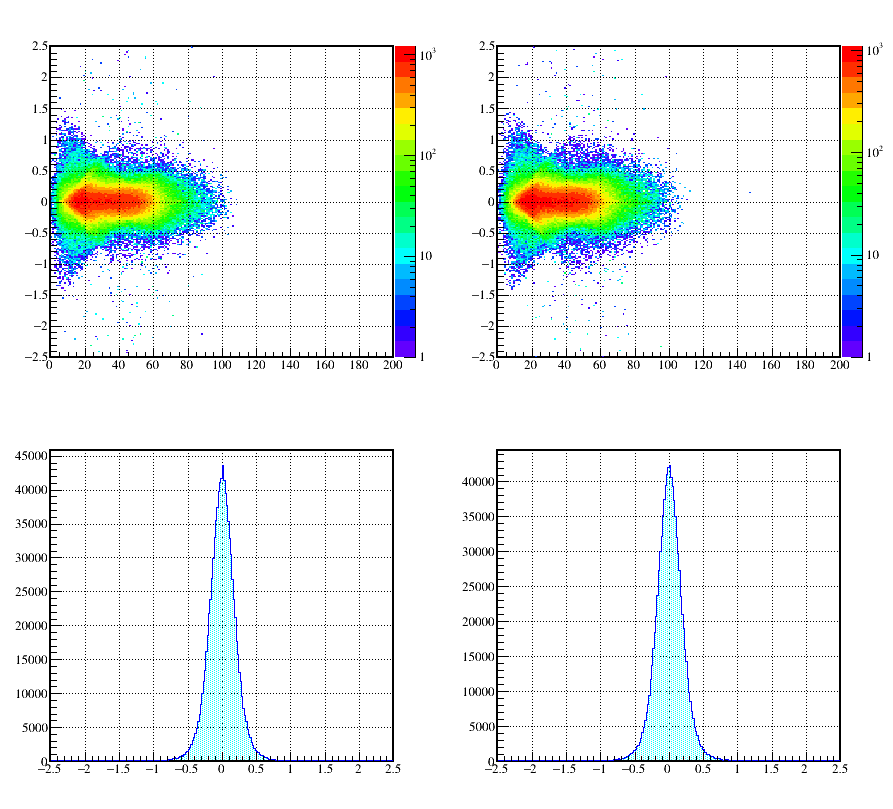
\includegraphics[width=14cm]{chapter4/BDC_residu.png}
    \caption[Tracking Residue Distribution of BDCs]{Tracking Residue Distribution of BDC1 (left) and BDC2 (right)}
    %\label{fig:residue_bdcs}
\end{figure}

\begin{table}
    \centering
    \begin{tabular}{c|cc}
    \hline
     & $\Delta_{x}$ [mm] & $\Delta_{y}$ [mm]\\
    \hline
    BDC1 & 0.1340 & 0.1627 \\
    BDC2 & 0.1422 & 0.1743 \\
    \hline \hline
    d& $\Delta_{a}$ [rad] & $\Delta_{b}$ [rad]\\
    \hline
    BDC1 & 0.01316 & 0.01330 \\
    BDC2 & 0.01396 & 0.01424 \\
    \hline
    \end{tabular}
    \caption{Position and Angular Resolution of BDCs}
    %\label{tab:resolution_bdcs}
\end{table}

\subsection{Beam Profile at Target}
The beam profile at the target is obtained by using the position information from BDCs. The position information ($x_{tgt}$, $y_{tgt}$) and angle information ($a_{tgt}$, $b_{tgt}$) at the target are obtained as,

\begin{align}
    x_{tgt} &= x_{BDC1} + \frac{(x_{BDC2} - x_{BDC1})}{L(BDC1 - BDC2)} \times L(BDC1 - tgt)\\
    y_{tgt} &= y_{BDC1} + \frac{(y_{BDC2} - y_{BDC1})}{L(BDC1 - BDC2)} \times L(BDC1 - tgt)\\
    a_{tgt} &= tan^{-1} \bigg( \frac{(x_{BDC2} - x_{BDC1})}{L(BDC1 - BDC2)} \bigg)\\
    b_{tgt} &= tan^{-1} \bigg( \frac{(y_{BDC2} - y_{BDC1})}{L(BDC1 - BDC2)} \bigg),
\end{align}
where the distance between BDCs is $L(BDC1 - BDC2) = 999.32 $mm, and the distance between BDC1 and the target is $L(BDC1 - tgt) = 2017.13$mm. The beam profile at the target is shown in Figure 4.4. 
\begin{figure}[h]
    \centering
    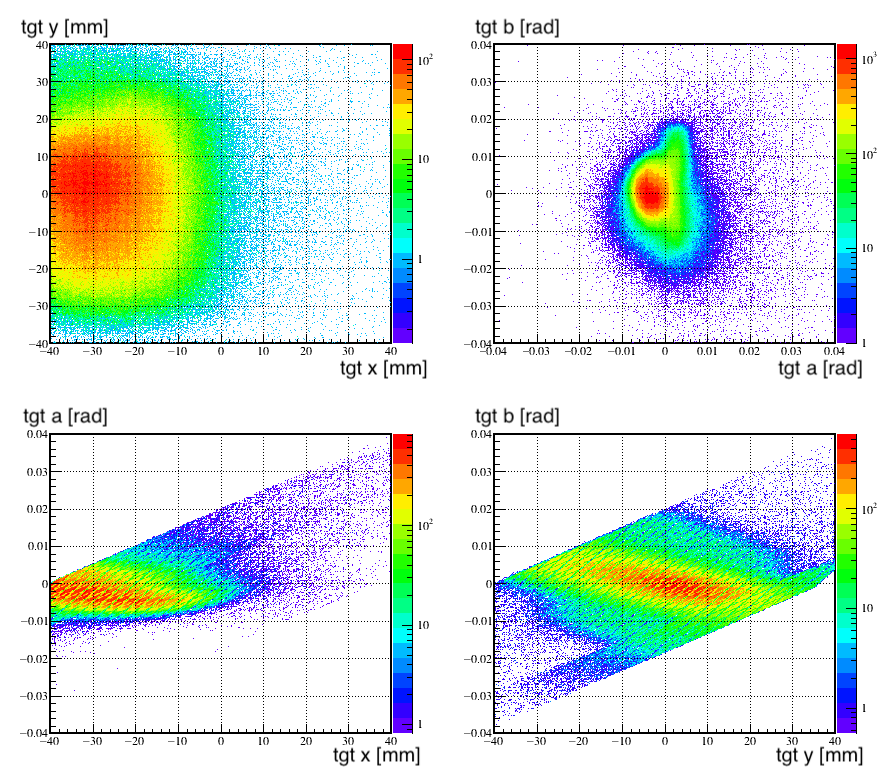
\includegraphics[width=10cm]{chapter4/target.png}
    \caption{${}^{17}$B Beam profile at target}
\end{figure}

%\subsection{Beam beta calculation}
%Invariant Mass를 계산하기 위해서는 Beam의 beta를 계산해야 한다. Beam의 beta는 다음과 같이 계산된다.

%\subsubsection{Eloss Calculation}
%Once $TOF_{F7-F13}$ has been calculated, the $\beta_{beam}$ can be calculated using the following equation. 

%\begin{align}
%    \beta_{F7-F13} = \frac{L(F7-F13)}{TOF_{F7-F13} \times c}
%\end{align}

%차후의 Invariant Mass 계산을 위해 target 중심에서의 beam-beta를 구할 필요가 있다. F5에서의 Brho를  beta는 tof713의 이차식으로 다음과 같이 나타낼 수 있다. 또한 각 특정 위치에 대한 coefficient는 표에 표시하였다.

%\begin{align}
%    TOF_{F7_Tgt} = a TOF_{F7-F13}^{2} + b TOF_{F7-F13} + c    \beta_{F5}  
%\end{align}

%\subsection{Efficiency of Upstream Detectors}

\clearpage

\subsection{FDC Calibration}
As same as BDC, FDC is also drift chamber. The tracking procedure is same as BDC. %The tracking residue distribution of FDC1 and FDC2 are shown in figure \ref{fig:residue_fdcs}. And the position and angular resolution of FDC1 and FDC2 are shown in table \ref{tab:resolution_fdcs}.
\begin{table}[h]
    \centering
    \begin{tabular}{c|cc}
        \hline
        &$t_{min}$ [ch]&$t_{max}$ [ch]\\
        \hline
        FDC1&1300&1700\\
        FDC2&500&1600\\        
        \hline
    \end{tabular}
    \caption[TDC Window Condition of FDCs]{TDC Window Condition of FDC1 (left) and FDC2 (right)}
\end{table}
\begin{figure}
    \centering
    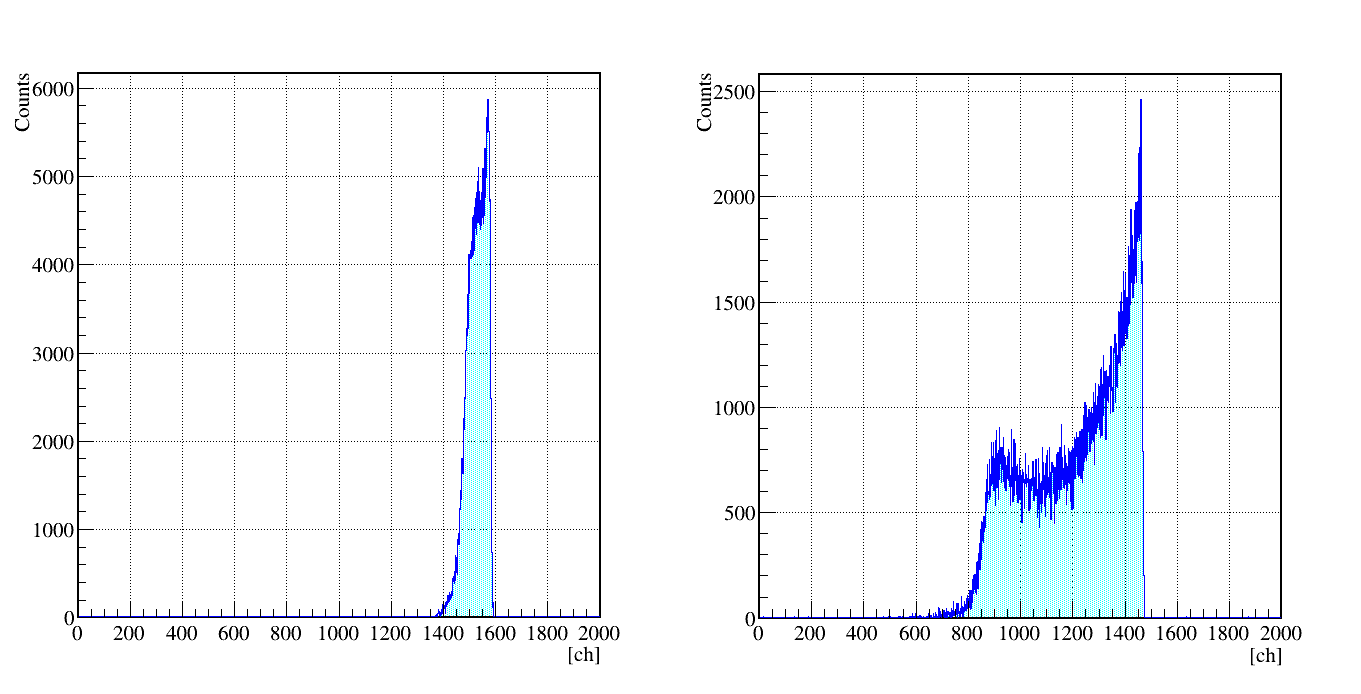
\includegraphics[width=14cm]{chapter4/tdc_fdcs.png}
    \caption[TDC Distribution of FDCs]{TDC Distribution of FDC1 (left) and FDC2 (right)}
\end{figure}


\section{Fragment Particle Identification}
Charged particle decayed from ${}^{17}$B is detected by the SAMURAI detector system. After reaction at secondary target, the secondary beam ${}^{17}$B is dissociated to charged particle ${}^{15}$B and two neutrons. The charged particle ${}^{15}$B bent by SAMURAI superconducting dipole magnet. Its trajectory is recorded by FDC1 and FDC2 before and after SAMURAI. And the energy loss and time of flight is measured by HODF plastic scintillator after FDC2.

\subsection{Analysis for Brho}
The Brho of the fragment is calculated from the position information of FDC1 and FDC2. 

\begin{align}
    &B\rho = f(x_{\text{FDC1}}, y_{\text{FDC1}}, a_{\text{FDC1}}, b_{\text{FDC1}}, x_{\text{FDC2}}, a_{\text{FDC2}})\\
    &a_{\text{FDC1}} = tan^{-1} \bigg( \frac{x_{\text{FDC1}} - x_{\text{tgt}}}{L(\text{FDC1 - Target})} \bigg)\\
    &b_{\text{FDC1}} = tan^{-1} \bigg( \frac{y_{\text{FDC1}} - y_{\text{tgt}}}{L(\text{FDC1 - Target})} \bigg)
\end{align}
The function of $B\rho$ is extracted by using TMultiDimFit class in ROOT using a trajectory obtained from Geant4 simulation. The simulation data input is the position and angle information of FDC1 and FDC2 in current experiment.

\subsection{Analysis for Time of Flight and Energy Loss}
\subsubsection{Analysis of Time of Flight}
Time of flight of charged particle is determined by the time difference between the HODF and the target. The time at target is determined by addition of the time at F13 and the time of flight from F13 to the target. The time of flight between F13 and the target is calculated with ${}1^{17}$B beam with Energy loss calculation considered the material between F13 and the target. The time of flight between HOD and target is defined by the following equation.

\begin{align}
    t_{\text{tgt}} = t_{F13} + tof_{\text{F13-tgt}}
    tof_{\text{HODF-tgt}} = t_{\text{HODF}} - t_{\text{tgt}} + \Delta t_{offset}
\end{align}
where $t_{\text{HOD}}$ is timing information of HODF and $\Delta t_{offset}$ is obtained by Geant4 simulation as same as $B\rho$ analysis. The $\Delta t_{offset}$ is 112.5256 ns.

\subsubsection{Analysis of Energy Loss}
In case of fragment, the energy loss is obtained from the light output information of HODF scintillator. From the Bethe-Bloch formula, we assumed that 
\begin{align}
    Z_{frag} \propto \beta_{frag} \sqrt{\Delta E} = \beta_{frag} \sqrt{Q_{\text{HOD}}}
\end{align}
Because of the proportional relation between $Z_{frag}$ and $\sqrt{Q_{\text{HOD}}}$, it is difficult to identify the fragment particle by only energy loss information. So first we gate the fragment particle by ${}^{17}$B beam, and assumed that most of fragment came from ${}^{17}$B should be ${}^{17}$B itself. Then we can get coefficient for calculating the Z.
\begin{align}
\end{align}

\subsection{Fragment Particle Identification}
Fragment particles are identified using the TOF-B$\rho$-$\Delta$E method as same as beam particle identification. TOF is calculated from time difference between target and HODF, B$\rho$ is calculated from the Geant4 simulation with FDC1 and FDC2 position information, and Z is calculated by HOD Q information. A/Z and Z is driven by the following equation.
\begin{align}
    \beta_{\text{frag}} &= L(\text{Target - HODF}) / ( {\text{TOF}}_{\text{Target - HODF}} \times c )\\
    A/Z &= c B\rho \gamma_{\text{frag}} / m_u \beta_{\text{frag}}\\
    Z &= p_0 + p_1 (Q_{\text{HOD}} - p_2 \frac{1}{\beta^2})
\end{align}
L(Target - HODF) is flight length from target to HODF. This is also calculated by Geant4 simulation with FDC1 and FDC2. The coefficient of Z calculation $p_0, p_1, p_2$ are obtained by linear fitting of HOD Q distribution. The fragment particle identification is shown in figure \ref{fig:fragpid_all} and \ref{fig:fragpid_b17}. Figure \ref{fig:fragpid_all} is the fragment particle identification of all events. Figure \ref{fig:fragpid_b17} is the fragment particle identification only from ${}^{17}$B beam events.

\begin{figure}
    \centering
    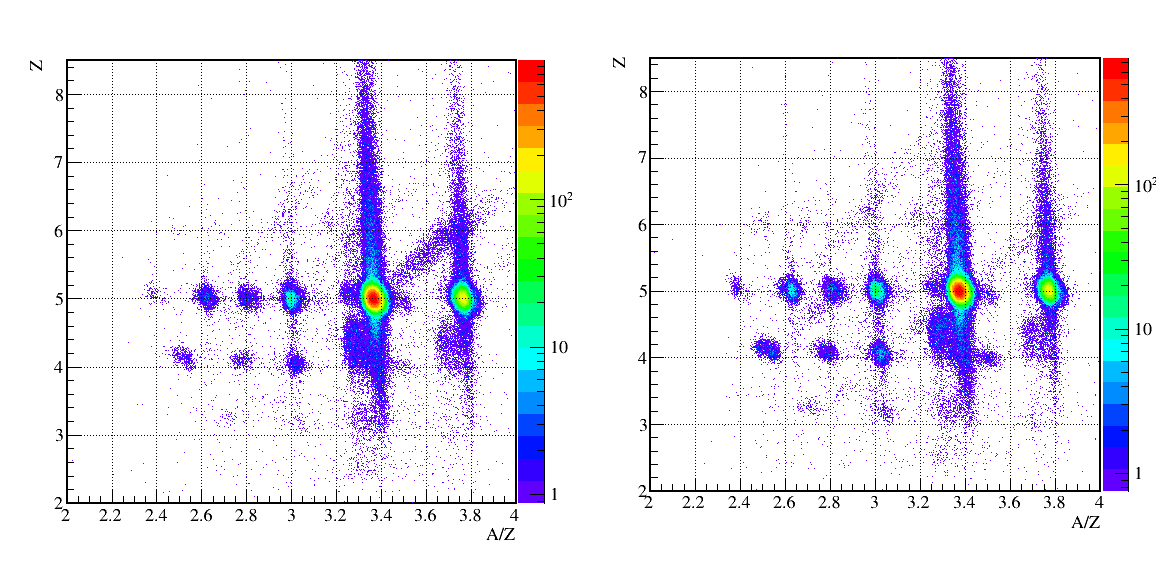
\includegraphics[width=14cm]{chapter4/fragpid_all.png}
    \caption[Fragment Particle Identification from All Secondary Beam]{Fragment Particle Identification of All Events at Pb target (left) and C target (right)}
    \label{fig:fragpid_all}
\end{figure}

\begin{figure}
    \centering
    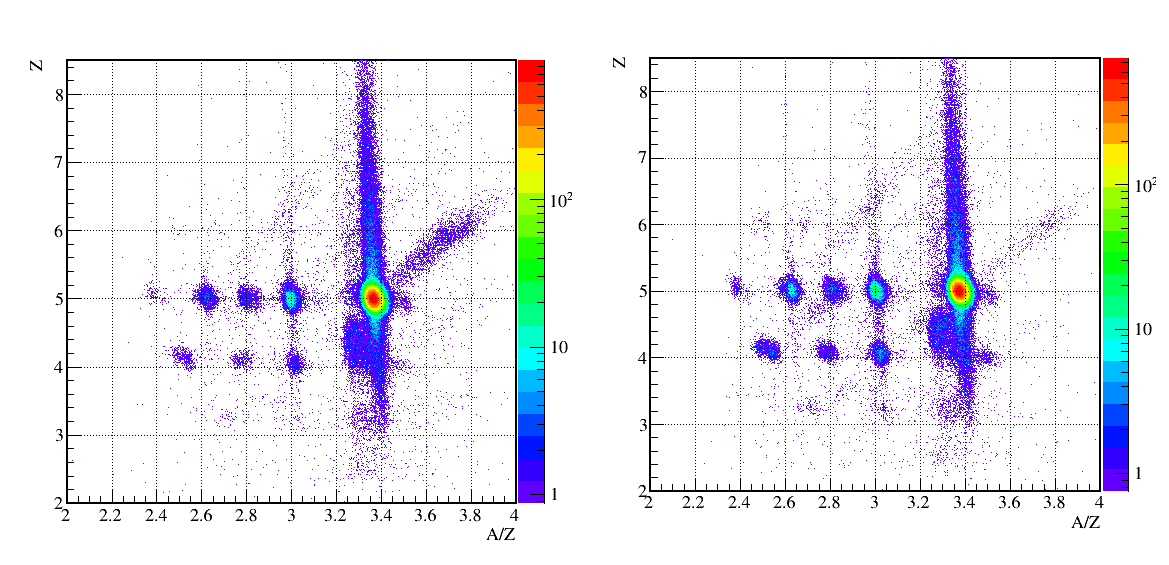
\includegraphics[width=14cm]{chapter4/fragpid_b17.png}
    \caption[Fragment Particle Identification from ${}^{17}$B Beam]{Fragment Particle Identification of ${}^{17}$B Events at Pb target (left) and C target (right)}
    \label{fig:fragpid_b17}
\end{figure}

\clearpage

\section{Analysis of Neutrons}
In this experiment, neutrons emitted from the secondary beam ${}^{17}$B are detected by the NEBULA neutron detector array. A neutron is detected indirectly by recoiled proton which is mainly produced by H($n$,$n$) and ${}^{12}$C($n$,$np$) reaction in the plastic-scintillator. Because of the indirect detection of neutrons, the selection of neutron events is more complicated than that of charged particles. The selection of neutron events is performed in four steps. First, reject the events which assumed as gamma event. Second, reject the events which is assumed as recoiled proton or gamma event. Third, in two neutron selection case, remove the event which is assumed as cross-talk. After all, select the fastest and second fastest event as a real neutron event. In following section, the detail of each step is described.

\subsection{Selection of One Neutron Events}
The selection of one neutron events is performed in three steps. 
\begin{enumerate}
    \item All events detected by the first VETO are considered to be charged particles and are rejected.
    \item Among the events detected by NEBULA, events with a light output Q of less than 6 MeVee are considered to be gamma rays and are rejected. In addition, events exceeding the maximum energy loss of a recoiled proton in one scintillator unit (130 MeVee) are also rejected.
    \item Events whose TOF from the target to the first wall is less than 40 ns and whose TOF from the target to the second wall is less than 42 ns are considered to be non-neutron events and are rejected.
\end{enumerate}
After these rejection procedure, we choose the fastest event as a real neutron event. 

\subsection {Selection of Two Neutron Events}
In the selection procedure of two neutron event, the rejection of charged particle and gamma ray is almost same with one neutron selection. But in case of selecting events of two neutrons, the most important process is the elimination of cross-talk. Cross-talk refers to the phenomenon where a single neutron generates multiple signals. Cross-talk is the most significant source of noise when selecting two-neutron events. The selection of two neutron events is performed in five steps. 
\begin{enumerate}
    \item All events detected by the first VETO are considered to be charged particles and are rejected.
    \item Among the events detected by NEBULA, events with a light output Q of less than 6 MeVee are considered to be gamma rays and are rejected. In addition, events exceeding the maximum energy loss of a recoiled proton in one scintillator unit (130 MeV) are also rejected.
    \item Events whose TOF from the target to the first wall is less than 40 ns and whose TOF from the target to the second wall is less than 42 ns are considered to be non-neutron events and are rejected.
    \item For events detected at the second VETO, detections in which the two fastest neutron events incident on the second NEUT wall are dr(xy) $<$ 500mm and 2ns $<$ dt $<$ 5ns are considered to be cluster scattering events from second VETO and are rejected.
    \item Cross-talk events are rejected.
\end{enumerate}
I will describe the three step of cross-talk rejection.

\subsubsection{Clustering event}
The clustering event means the two events which are detected in very close distance in very small time interval. It means the second event is likely to be a recoil proton from the first event. The clustering event is rejected by the following condition.
\begin{align}
    \bigg( \frac{dr-dr_0}{3\sigma_{dr}} \bigg)^2 + \bigg( \frac{dt-dt_0}{3\sigma_{dt}} \bigg)^2 < 1 
\end{align}
where $dr$ and $dt$ are the position and time difference between two events. And $dr_0$ and $dt_0$, $\sigma_{dr}$ and $\sigma_{dt}$ mean the central values and the standard deviations of the distribution of $dr$ and $dt$ for the clustering events. The $dr_0$ and $dt_0$ are 98.35 mm and 0.65 ns, and $\sigma_{dr}$ and $\sigma_{dt}$ are 71.07 mm and 0.40 ns. 

\subsubsection{same wall event}

\subsubsection{different wall event}


To reject cross-talk, a Geant4 simulation was performed to generate events of ${}^{16}\text{B} \to {}^{15}\text{B}+n$, thereby replicating cases where all two-neutron events are due to cross-talk. The details of the executed Geant4 simulation are as follows.

\begin{center}
    \begin{tabular}[h]{c|c}
        \hline \hline
        Reaction & ${}^{16}\text{B} \to {}^{15}\text{B}+n$ \\
        Beam Energy & 270 MeV/u\\
        Relative Energy & 0 - 10 MeV (Uniformly Generated)\\
        Position Distribution & Reconstructed from ${}^{17}$B Beam profile\\
        Angular Distribution & Reconstructed from ${}^{17}$B Beam profile \\
        \hline \hline
    \end{tabular}
\end{center}

\section{Cross-talk Residual Rate}
Even though we performed the cross talk rejection, there probably be residual of cross talk. For each cross talk step, we evaluated the residual rate of cross talk. Each step is as follows.
\begin{enumerate}
    \item (a) no rejection
    \item (b) clustering rejection
    \item (c) clustering rejection + same wall rejection
    \item (d) clustering rejection + same wall rejection + gamma rejection
\end{enumerate}
The residual rate of cross talk can be calculated by the following formula.
\begin{align}
    R = \frac{N_{M>2}}{N_{M>1}}
\end{align}
The result is the multiplicity M $\>$ event is 225385, and M>2 event of each step and residual rate R are in table 4.7.
\begin{table}[h]
    \centering
    \begin{tabular}[h]{c|c|c|c}
        \hline
        Condition & same wall event (R) & different wall event (R) & all wall event (R)\\
        \hline
        (a) & 89721 (39.8$\%$) & 10123 (4.5$\%$) & 99844 (44.3$\%$) \\
        (b) & 29032 (12.9$\%$) & 16848 (7.5$\%$) & 45880 (20.4$\%$)\\
        (c) & 6274 (2.8)$\%$)   & 2791 (1.2$\%$)& 9065 (4.0$\%$)\\
        (d) & 5352 (2.4$\%$)& 2089 (0.9$\%$)& 7441 (3.3$\%$)\\
        \hline
    \end{tabular}
    \caption{The cross talk residual rate evaluation}
\end{table}

\section{Acceptance and Efficiency Correction}
For evaluating the two-neutron detection efficiency and SAMURAI acceptance, the simulation is performed by Geant4. The information of simulation is as follows.

\begin{center}
    \begin{tabular}[h]{c|c}
        \hline
        Physics Model & Phase Space Decay \\
        Reaction & ${}^{17}\text{B} \to {}^{15}\text{B} + 2n$\\
        Beam Energy & 270 MeV/u\\
        Relative Energy & 1-10 MeV (Uniformly generated)\\
        Scattering Angle & 0-30 mrad (Uniformly generated)\\
        \hline
    \end{tabular}
\end{center}

The result of simulation is shown in figure \ref{fig:acc_same_diff}.
\begin{figure}
    \centering
    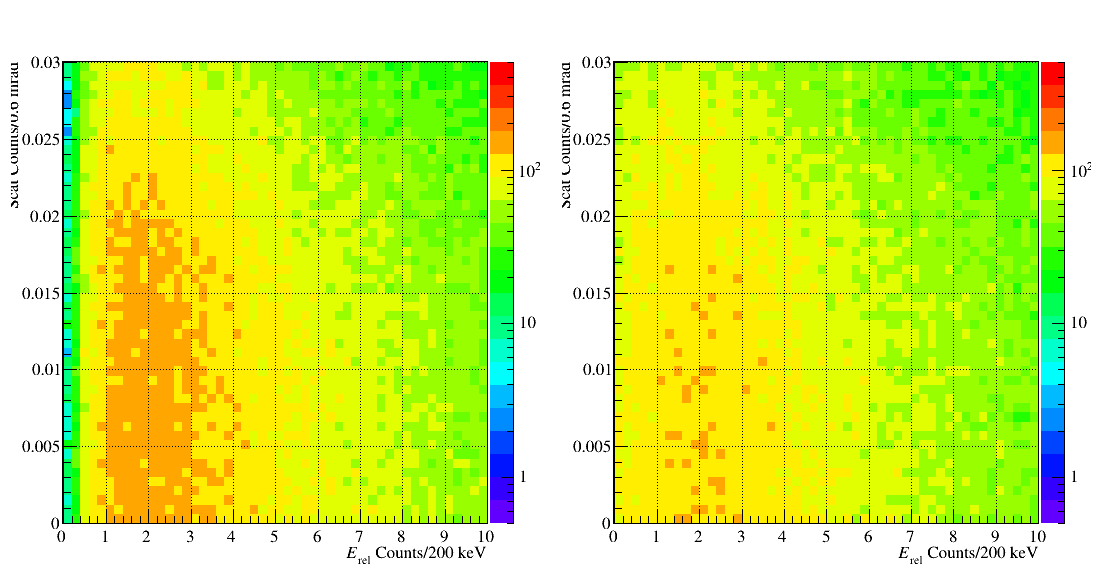
\includegraphics[width=14cm]{chapter4/acc_same_diff.png}
    \caption[$2n$ Acceptance for $E_{rel}$ and $\theta_{scat}$]{2n Acceptance for same wall (left) and different wall (right)}
    \label{fig:acc_same_diff}
\end{figure}


\section{Reconstruction of Invariant Mass}
After identification of all fragments from the ${}^{17}$B beam, the invariant mass of the system can be reconstructed. First, the beam vector is reconstructed by $\beta_{\text{Beam}}$ and beam profile at target. $\beta_{\text{Beam}}$ is calculated using Eloss code, considering the energy loss from F5 slit to the middle of target.
\begin{align}
    %\gamma_{\text{Beam}} &= \frac{1}{\sqrt{1-\beta_{\text{Beam}}^{2}}}\\
    P_z ({}^{17}\text{B}) &=  m({}^{17}\text{B}) \gamma_{\text{Beam}} \frac{1}{\sqrt{1+tan^2(tgta)+tan^2(tgtb)}}\\
    P_x ({}^{17}\text{B}) &=  P_z ({}^{17}\text{B}) \cdot \tan(tgta)\\ 
    P_y ({}^{17}\text{B}) &=  P_z ({}^{17}\text{B}) \cdot \tan(tgtb)
\end{align}
Second, the momentum of the ${}^{15}$B fragment is calculated from the 
\begin{align}
    \vec{P} ({}^{15}\text{B}) &= B\rho c Z \\
    E ({}^{15}\text{B}) &= \sqrt{m({}^{15}\text{B})^{2} + P({}^{15}\text{B})^{2}}\\
    \vec{P_z} ({}^{15}\text{B}) &= \vec{P} \frac{1}{\sqrt{1 + \tan^2(scata)+ \tan^2(scatb)}}\\
    \vec{P_x} ({}^{15}\text{B}) &= \vec{P_z} ({}^{15}\text{B}) \cdot \tan(scata)\\
    \vec{P_y} ({}^{15}\text{B}) &= \vec{P_z} ({}^{15}\text{B}) \cdot \tan(scatb)
\end{align}
Finally the neutron vector is reconstructed by the position information from NEBULA and the time-of-flight as (4.34). From these three vectors, the invariant mass of the system is calculated.
The momentum $P(n)$ of the neutron is reconstructed from the detection position in NEBULA relative to the target, and the time-of-flight (TOF). The momentum vector of the neutron is described as follows.

\begin{align}
    L &= | \vec{r}_{\text{tgt}} - \vec{r}_{n} | \\
    \beta_{n} &= L / (\text{TOF}_{\text{NEB-tgt}} \times c) \\
    P_{n} &= m_{n} \beta_{n} \gamma_{n} \\
    E_{n} &= m_{n} \gamma_{n} \\
    \vec{P_{n}} &= \frac{\vec{r_{n}} - \vec{r_{tgt}}}{L} P_{n}
\end{align}
where, $\vec{r}_{\text{tgt}}$ is the position of the target $\vec{r}_{\text{tgt}}$, $m_{n}$ is the neutron mass


\section{Relative Energy Spectrum}

\begin{figure}[h]
    \centering
    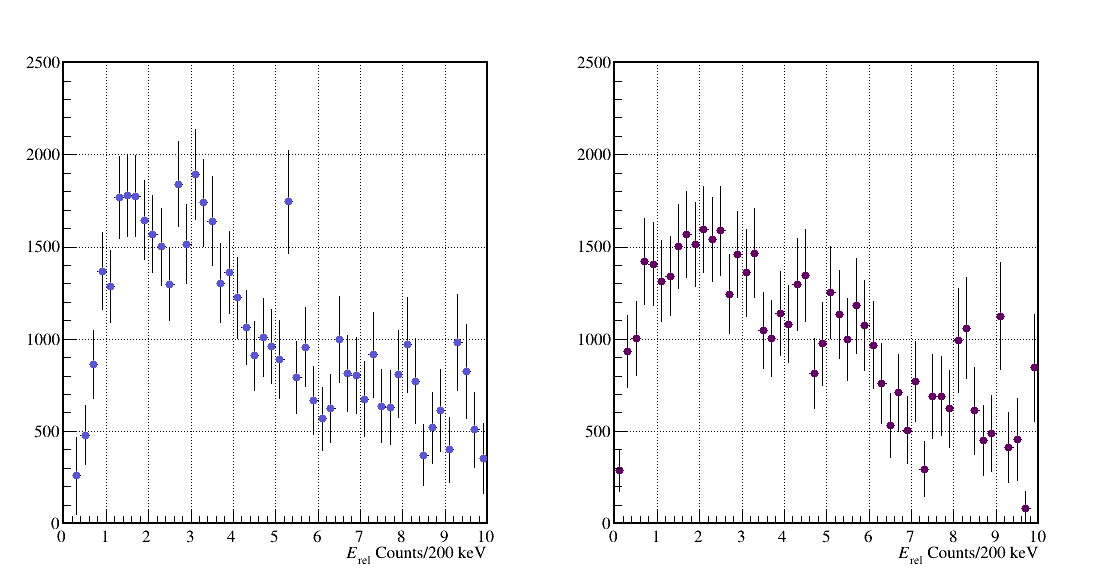
\includegraphics[width=14cm]{chapter4/Pb_same_diff.png}
    \caption{Relative Energy Spectrum of ${}^{15}\text{B} + 2n$ at Pb target}
\end{figure}
\begin{figure}[h]
    \centering
    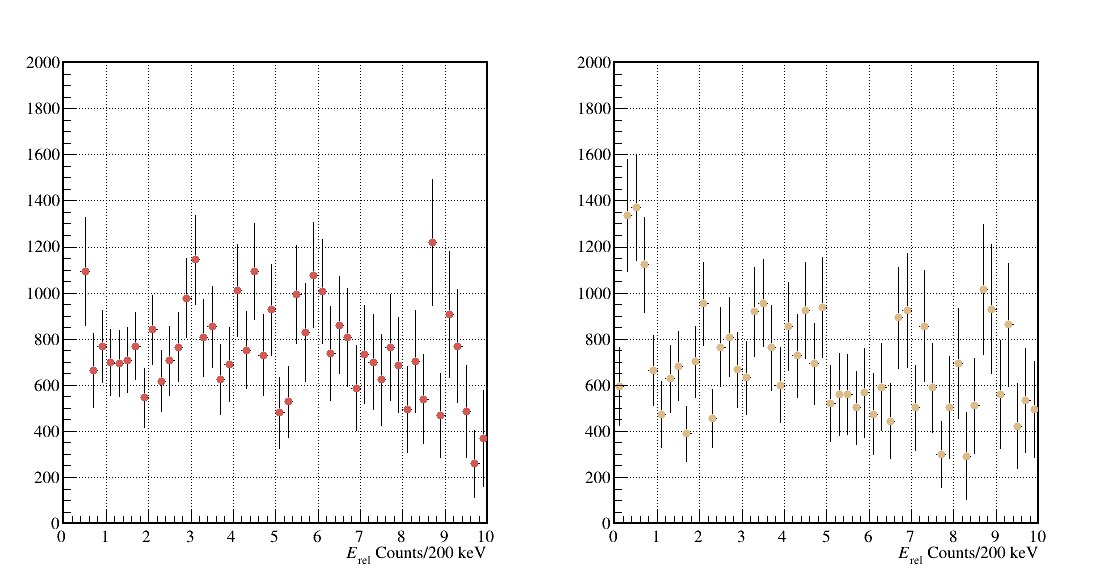
\includegraphics[width=14cm]{chapter4/C_same_diff.png}
    \caption{Relative Energy Spectrum of ${}^{15}\text{B} + 2n$ at C target}
\end{figure}

%\begin{figure}
%    \centering
%    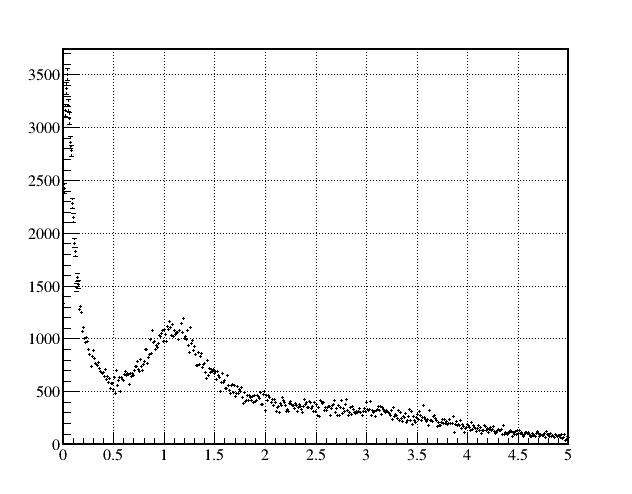
\includegraphics[width=14cm]{chapter4/16Bn_C.png}
%    \caption{Relative Energy Spectrum of ${}^{16}\text{B} + n$ at C target}
%\end{figure}
